\documentclass{article}
\usepackage[%
    left=0.5in,%
    right=0.5in,%
    top=0.5in,%
    bottom=0.5in,%
]{geometry}%
\usepackage{minitoc}
\usepackage{multicol}
\usepackage{graphicx}
\graphicspath{ {./} }

\begin{document}
\section{Threads}

\subsection{Theads from an OS perspective}
\begin{flushleft}
A proces consists of two \textbf{fundamental units}
\begin{itemize}
	\item \textbf{Resources}: all related resources are grouped together:
	\begin{itemize}
		\item A logical addres space containing the process image (program, data, heap stack)
		\item Files, I/O devices, I/O channels
	\end{itemize}
	\item \textbf{Execution trace}, i.e, an entity that gets exceuted
\end{itemize}
A process can \textbf{share its resources} between \textbf{multiple execution traces}. Every thread has its own \textbf{execution context} (e.g program counter, stack, registers).\\
All threads have \textbf{access} to the process \textbf{shared resources}
\begin{itemize}
	\item E.g files, one thread opens a file, all threads on the same process can acess the file
	\item Global variables, memory, etc. Which is needed or synchronisation
\end{itemize}
Some CPUs (hyperthreaded ones) have direct \textbf{hardware support} for \textbf{multi-threading}. They can offer up to 8 hardware threads per core.
\end{flushleft}
\bigskip


\begin{multicols}{2}
Similar to processes, threads have:
\begin{itemize}
	\item \textbf{States} and \textbf{transitions} (new, running, blocked, ready, terminated)
	\item \textbf{A thread control block}
\end{itemize}
Threads incur \textbf{less overhead} to create/terminate/switch (address space remains the same for threads of the same process)
\smallskip
\begin{center}
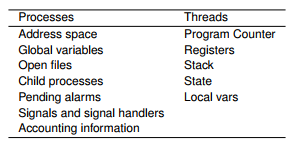
\includegraphics[scale=0.5]{Selection_007.png}
\end{center}
\end{multicols}

\begin{itemize}
	\item \textbf{Inter-thread communication} is easier/faster than \textbf{interprocess} communication (threads share memory by default)
	\item \textbf{No protection boundaries} are required in the address space. Threads are cooperating, belong to the same user, and have a common goal)
	\item \textbf{Synchronisation} has to be considered carfully
\end{itemize}

\subsection{Why use threads}
\begin{flushleft}
Multiple \textbf{related activites} apply to the \textbf{same resources}, these resources should be accessible/shared\\
Processes will often contain multiple \textbf{blocking tasks}
\begin{itemize}
	\item I/O operations (thread blocks, \textbf{interrupt} marks completion)
	\item Memory access: pages faults are result in blocking
\end{itemize}
Such activities should be carried out in \textbf{parallel/concurrently}. \textbf{Application examples}: webservers, make program, spreadsheets, word processors, processing large data volumes
\end{flushleft}
\end{document}
